% Weekly research report — 2026-07-28 — the data-scale curve.
% Build: make figures (once, pulls HF artifacts) && make.
% Every number in the prose is a macro from generated/numbers.tex (derived from the run
% artifacts on HF) — nothing below is hand-typed data.
\documentclass[11pt]{article}
\usepackage{weeklyreport}
% AUTO-GENERATED by make_figures.py from runs/curve.csv + runs/*/metrics.csv on HF.
% Every number quoted in the report's prose lives here. Do not edit by hand.
\newcommand*\cdAtwenty{23.68}
\newcommand*\cdBtwenty{25.02}
\newcommand*\cdCtwenty{25.25}
\newcommand*\gapCtwenty{6.6}
\newcommand*\gapBtwenty{5.7}
\newcommand*\cmseBtwenty{0.085}
\newcommand*\cdAsixty{19.91}
\newcommand*\cdBsixty{20.83}
\newcommand*\cdCsixty{20.86}
\newcommand*\gapCsixty{4.8}
\newcommand*\gapBsixty{4.6}
\newcommand*\cmseBsixty{0.078}
\newcommand*\cdAonefifty{18.56}
\newcommand*\cdBonefifty{19.24}
\newcommand*\cdConefifty{19.31}
\newcommand*\gapConefifty{4.0}
\newcommand*\gapBonefifty{3.7}
\newcommand*\cmseBonefifty{0.073}
\newcommand*\gapCseedOne{3.7}
\newcommand*\gapCseedTwo{4.1}
\newcommand*\gapCseedThree{4.3}
\newcommand*\fsAonefifty{0.46}
\newcommand*\fsConefifty{0.44}
\newcommand*\fsBonefifty{0.44}
\newcommand*\cdAonefiftyLo{18.35}
\newcommand*\cdAonefiftyHi{18.83}
\newcommand*\cmseNN{0.082}
\newcommand*\cmseMean{0.070}
\newcommand*\cmseMedian{0.081}
\newcommand*\cmseOracle{0.020}
\newcommand*\nBundles{600}
\newcommand*\nRuns{15}
\newcommand*\nTrainLow{60}
\newcommand*\nTrainMid{180}
\newcommand*\nTrainTop{433}
\newcommand*\totalEpochs{1595}
\newcommand*\epochsMin{65}
\newcommand*\epochsMax{145}
\newcommand*\datasetRev{0db547ff6b}


\reporttitle{Does per-point color help point-cloud completion?\\The data-scale curve}
\reportweek{2026-07-28}
\reportdates{21--28 July 2026}
\reportauthors{Efe Yenice (researcher) \textperiodcentered\ Claude (AI co-researcher)}
\reportquestion{does the geometry penalty from per-point color input shrink---or flip---as training data grows?}
\reportrepo{\texttt{github.com/efeyenice/point-cloud-completion-research} \textperiodcentered\ \texttt{reports/2026-07-28-scale-curve}}

\begin{document}
\reportheader

\begin{tldr}
\begin{enumerate}
  \item \textbf{The color-input harm shrinks with data, but does not flip.} Feeding
  per-point RGB into the completion network still hurts geometry at every tested scale:
  the \arm{C\_colin}-vs-\arm{A\_geo} test CD-L1 gap falls from \worse{\gapCtwenty} at
  $N{=}20$ models/category to \worse{\gapCsixty} at $N{=}60$ and \worse{\gapConefifty} at
  $N{=}150$ (mean of 3 seeds; every seed agrees on the sign:
  \gapCseedOne--\gapCseedThree\,\%). The trend supports the small-data-artifact
  hypothesis, but no crossover has been observed yet (\cref{fig:curve}).
  \item \textbf{Predicting color stays free --- the cost is the input, not the output.}
  \arm{B\_joint} (which also \emph{outputs} color) matches or slightly beats
  \arm{C\_colin} on geometry at every rung (\worse{\gapBonefifty} vs.\
  \worse{\gapConefifty} at $N{=}150$). Its learned color head now beats the NN-copy
  (\cmseBonefifty{} vs.\ \cmseNN{} MSE) and median-copy baselines, but still loses to the
  trivial \emph{mean-copy} baseline (\cmseMean); color prediction quality is the next
  open gap (\cref{fig:color}).
  \item \textbf{The pipeline is now disconnect-proof, and that is what made the week
  possible:} \nBundles{} freshly generated model bundles and \nRuns{} training runs
  (\totalEpochs{} epochs total) streamed to Hugging Face with per-unit atomic commits and
  idempotent resume; Colab disconnects and VM recycles cost at most one unit of work.
\end{enumerate}
\end{tldr}

\section{The story so far}\label{sec:story}

The project asks one controlled question: \emph{does adding per-point RGB color improve
point-cloud completion, and under what conditions?} The cross-modal literature says color
helps a lot --- but in a different setting: methods like EGIInet inject a separate,
complete \emph{guidance image} ($\sim$58\,\% CD reduction over geometry-only baselines).
Our setting is stricter and unstudied: the color rides \emph{on the partial points
themselves} (and, in one arm, must also be \emph{predicted} for the completed cloud).

To isolate color's effect we train one from-scratch PCN backbone in three arms that
differ only in their input/output channels:

\begin{center}\small
\begin{tabular}{llll}
\toprule
arm & input & output & role \\
\midrule
\arm{A\_geo}   & xyz    & xyz    & geometry baseline \\
\arm{B\_joint} & xyzrgb & xyzrgb & does \emph{outputting} color cost geometry? \\
\arm{C\_colin} & xyzrgb & xyz    & does color \emph{input} help geometry? \\
\bottomrule
\end{tabular}
\end{center}

The first controlled result (previous report, $\sim$15 models/category) was the opposite
of the literature: color input \emph{hurt} geometry by $\sim$17\,\%, most plausibly
because at tiny scale per-point color acts as a per-model fingerprint that eases
memorization instead of generalization. That made \textbf{data scale the binding
constraint}, and this week's question follows directly: \emph{track the harm as a
function of training-set size $N$} --- if it is a small-data artifact, it should shrink,
and eventually flip (ADR-0007).

\section{What we did this week}\label{sec:did}

\subsection{The experiment: a data-scale curve}\label{sec:design}

Train all three arms at $N \in \{20, 60, 150\}$ models per category (airplane, car,
chair) and read the \arm{C}-vs-\arm{A} gap as a function of $N$. Design choices that make
the curve trustworthy:

\begin{itemize}
  \item \textbf{One variable.} A \emph{fixed held-out test set} (30 models/category,
  never trained on, reserved before any training) is scored at every rung, and the
  training pools are \emph{nested} ($N{=}20 \subset 60 \subset 150$), so $N$ is the only
  thing that changes along the curve. A fixed validation set (15/category) drives
  checkpoint selection and early stopping (patience 25 epochs, validated every 10, budget
  300).
  \item \textbf{Seeds where they matter.} The top rung --- where the claim lives --- runs
  3 seeds per arm; lower rungs run 1 (ADR-0007's cost/precision trade).
  \item \textbf{Baselines that give color numbers meaning.} Three training-free
  color-copy predictors (NN-copy, mean-copy, median-copy from the partial input) plus the
  NN-\emph{oracle} floor bracket the learned color head from below and above.
  \item \textbf{Same generation for every model.} \nBundles{} bundles regenerated from
  scratch with the colored sampling pipeline (dense EPFL colored cloud
  $\rightarrow$ color-aware 8192-point GT $\rightarrow$ 8 seeded \texttt{meshray\_nn}
  partial views; 4 views per model used in training). Fully textureless models are
  dropped (color std $\le 0.01$), leaving \nTrainTop{} of 450 pool models at the top
  rung.
\end{itemize}

\subsection{The ops overhaul that made it runnable}\label{sec:ops}

Last week's runs kept dying with Colab disconnects: results lived in Python lists,
intermediates on the VM's ephemeral disk, and a death at 99\,\% cost 100\,\%. This week
we rebuilt the operational layer around one rule (ADR-0008): \textbf{``done'' means bytes
on Hugging Face, never ``in RAM''} --- every long job commits per unit and resumes
idempotently.

\begin{center}
\begin{tikzpicture}[
  node distance=7mm and 8.5mm,
  box/.style={draw=wrnavy, rounded corners=1.5pt, fill=wrnavy!5, font=\scriptsize,
              align=center, inner sep=3pt, minimum height=8mm},
  store/.style={box, fill=wraccent!12},
  lab/.style={font=\tiny\itshape, color=wrgray, align=center},
  arr/.style={-{Stealth[length=2mm]}, thick, color=wrnavy}]
  \node[store] (sn) {ShapeNet\\(HF)};
  \node[box, right=of sn] (gen) {\texttt{partialGen}\\Colab GPU};
  \node[store, right=of gen] (data) {HF \texttt{data/}\\atomic \texttt{npz}/model};
  \node[box, right=of data] (train) {\texttt{pcnTraining}\\Colab GPU};
  \node[store, right=of train] (runs) {HF \texttt{runs/}\\ckpt every 10\,min};
  \node[store, below=4.5mm of train, xshift=-16mm] (wandb) {W\&B (live metrics)};
  \draw[arr] (sn) -- (gen);
  \draw[arr] (gen) -- (data);
  \draw[arr] (data) -- (train);
  \draw[arr] (train) -- (runs);
  \draw[arr] (train.south) -- (wandb.east);
  \draw[arr, dashed] (runs.south) to[bend left=28]
    node[lab, below=0.2mm] {resume} (train.south);
\end{tikzpicture}
\end{center}

Concretely: the data generator writes one atomic \texttt{\{model\_id\}.npz} per model and
a background scheduler streams it to the HF dataset (a crash costs one model; re-running
the cell skips everything already uploaded); training streams checkpoints and
\texttt{metrics.csv} to HF every 10 minutes and logs live to W\&B; the curve driver
resumes mid-run after a VM recycle by reloading prior state from HF. Code lives in git
only (notebooks output-stripped); Google Drive is fully retired. The week's runs were
completed across multiple Colab sessions with no lost work.

\section{Results}\label{sec:results}

\begin{figure}[t]
  \centering
  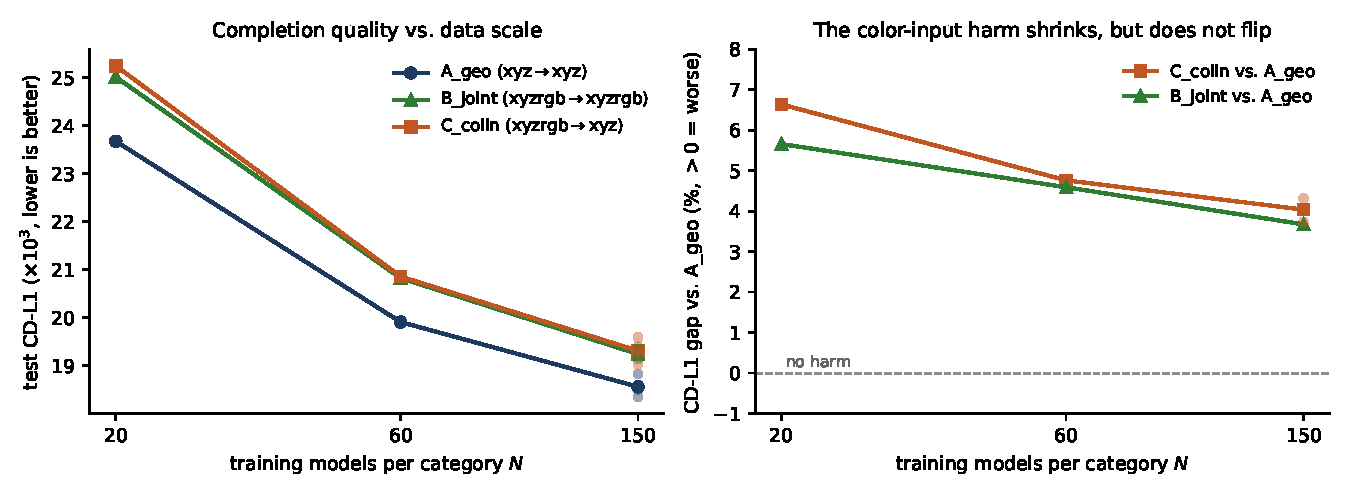
\includegraphics[width=\textwidth]{figures/fig_curve.pdf}
  \caption{\textbf{The data-scale curve} on the fixed held-out test set (90 shapes).
  Left: absolute test CD-L1 per arm vs.\ training models per category $N$; faint points
  are the individual seeds at $N{=}150$. Right: the same data as a gap relative to
  \arm{A\_geo}; positive means color made geometry worse. The harm shrinks monotonically
  (\worse{\gapCtwenty} $\rightarrow$ \worse{\gapCsixty} $\rightarrow$
  \worse{\gapConefifty}) but stays positive at every tested scale.}
  \label{fig:curve}
\end{figure}

\subsection{The headline: harm vs.\ scale}\label{sec:headline}

\Cref{fig:curve} and \cref{tab:rungs} carry the week's answer. All arms improve steeply
with data ($\cdAtwenty \rightarrow \cdAonefifty$ CD-L1 for \arm{A\_geo} alone --- data
remains the dominant lever for everything). Within-rung, the ordering never changes:
\arm{A\_geo} best, both color-input arms behind. The gap narrows with every step of $N$
--- consistent with the memorization-fingerprint account --- but at $N{=}150$/category it
is still \worse{\gapConefifty}, and \emph{every} top-rung seed pairing agrees on the sign
(\gapCseedOne, \gapCseedTwo, \gapCseedThree\,\%). F-score tells the same story
(\fsAonefifty{} vs.\ \fsConefifty{} at $N{=}150$). We therefore report: \textbf{the harm
behaves like a small-data artifact, but has not vanished at the scales we can currently
reach}. No extrapolated crossover is claimed from three points.

\begin{table}[h]
  \centering\small
  \begin{tabular}{rrrrrrrr}
    \toprule
    $N$/cat & train models & \arm{A\_geo} & \arm{C\_colin} & \arm{B\_joint} &
    C vs.\ A & B vs.\ A & B color MSE \\
    \midrule
    20  & \nTrainLow  & \cdAtwenty{}   & \cdCtwenty{}   & \cdBtwenty{}   & +\gapCtwenty\,\%   & +\gapBtwenty\,\%   & \cmseBtwenty{} \\
    60  & \nTrainMid  & \cdAsixty{}    & \cdCsixty{}    & \cdBsixty{}    & +\gapCsixty\,\%    & +\gapBsixty\,\%    & \cmseBsixty{} \\
    150 & \nTrainTop  & \cdAonefifty{} & \cdConefifty{} & \cdBonefifty{} & +\gapConefifty\,\% & +\gapBonefifty\,\% & \cmseBonefifty{} \\
    \bottomrule
  \end{tabular}
  \caption{Test CD-L1 ($\times 10^3$, lower is better; $N{=}150$ row averages 3 seeds)
  and the gaps relative to the geometry baseline. Copy-baseline color MSEs for
  comparison: NN \cmseNN{}, median \cmseMedian{}, mean \cmseMean{}; oracle floor
  \cmseOracle. Full per-run table in \cref{app:runs}.}
  \label{tab:rungs}
\end{table}

\subsection{The color head vs.\ its baselines}\label{sec:color}

\begin{figure}[h]
  \centering
  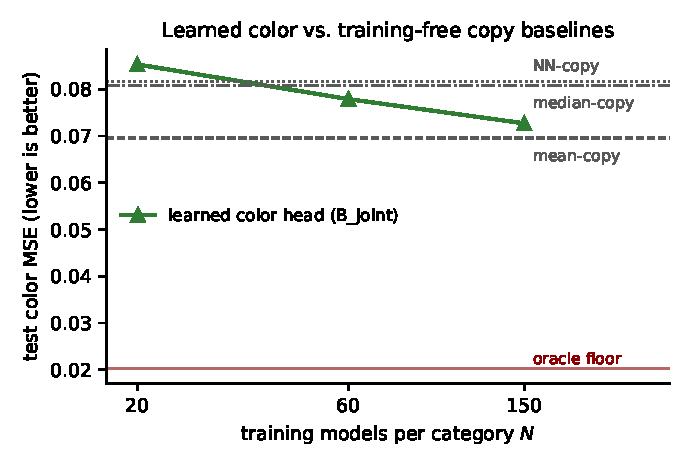
\includegraphics[width=0.62\textwidth]{figures/fig_color.pdf}
  \caption{\textbf{Learned color vs.\ training-free baselines} (test color MSE at the
  GT's nearest predicted point). The learned head improves with data and has passed
  NN-copy and median-copy, but not yet the mean-copy baseline; the oracle floor
  (\cmseOracle) shows most of the headroom is still unclaimed.}
  \label{fig:color}
\end{figure}

Two honest reads. First, the \emph{geometry} cost of adding the color \emph{output} is
zero: \arm{B\_joint} lands at or slightly ahead of \arm{C\_colin} at every rung
(\cref{tab:rungs}), so predicting color is not what hurts --- ingesting it is. Second,
the color the head predicts is still weak: it has learned enough to beat copying colors
from the partial (NN-copy, \cmseNN) but not enough to beat answering ``the average
color of this object'' (mean-copy, \cmseMean{} vs.\ learned \cmseBonefifty{} at
$N{=}150$). The qualitative panels (\cref{fig:panels}, right column) show why: under an
MSE-reported, BCE-trained objective the head hedges toward washed-out, low-saturation
colors. Improving this head --- including the advisor's Gaussian-distribution ideas ---
is a concrete next thread, and the copy baselines now give it a meaningful bar to clear.

\subsection{Qualitative check}\label{sec:qual}

\begin{figure}[t]
  \centering
  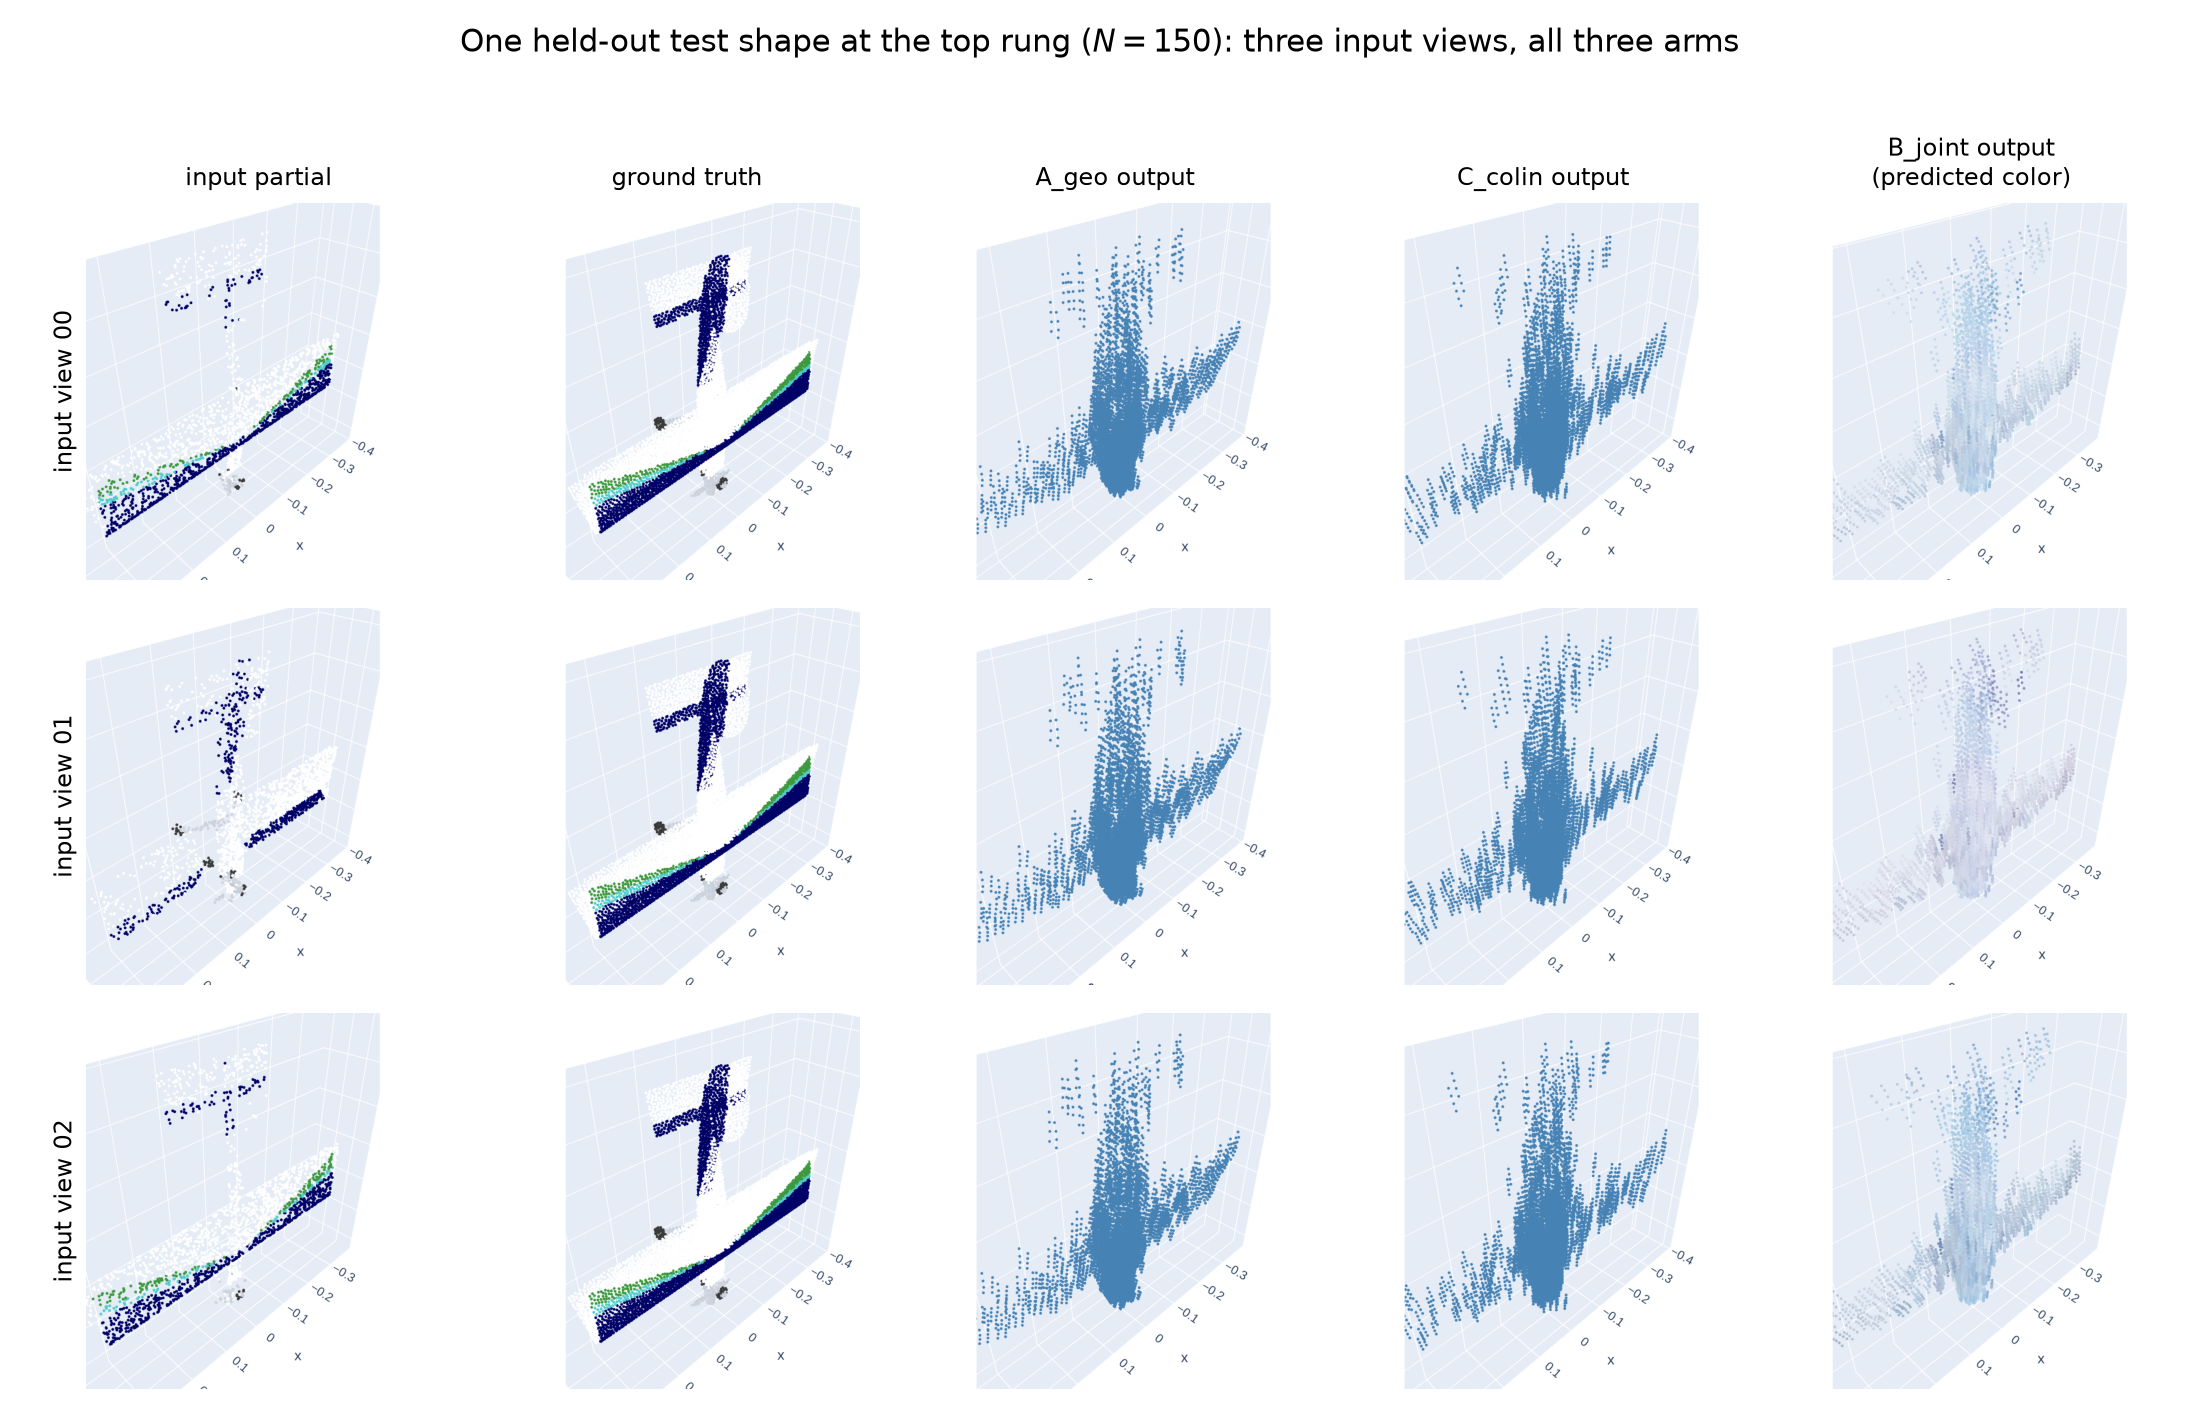
\includegraphics[width=\textwidth]{figures/fig_panels.png}
  \caption{\textbf{One held-out test airplane at $N{=}150$}, three input views (rows),
  recomposed from the run's own renders. Columns: input partial, colored GT, and each
  arm's fine output (8192 points; \arm{B\_joint}'s shown in its predicted colors).
  Completions are recognizable but coarse at this scale, and \arm{B}'s predicted colors
  are visibly desaturated --- the regression-to-the-mean behavior behind
  \cref{fig:color}.}
  \label{fig:panels}
\end{figure}

\Cref{fig:panels} keeps us honest about absolute quality: at $N{=}150$/category the
completions capture the coarse shape but none of the fine structure. That is expected ---
the PCN literature trains on $\sim$30{,}000 models, two orders of magnitude more than our
largest rung --- and it is why every claim in this report is \emph{relative,
within-pipeline}: same data, same splits, same budget, arms differing only in color
channels. The training curves (\cref{app:training}) show the same thing quantitatively:
in all \nRuns{} runs validation plateaus early while train keeps improving --- the
classic data-limited signature, at every rung we can afford.

\subsection{Continuity with the previous result}\label{sec:continuity}

The prior report measured the harm at $\sim$17\,\% ($\sim$15 models/category); this
pipeline's smallest rung ($N{=}20$) measures \worse{\gapCtwenty}. The sign and the
``harm at small $N$'' conclusion replicate; the magnitude does not, and we flag that
plainly. Between the two measurements the pipeline changed in ways that all plausibly
shrink the measured gap: a fixed, larger held-out test set (30/category vs.\ ad-hoc);
early stopping on validation (the old fixed-epoch training let arms overfit for
different lengths); one partial-generation method (\texttt{meshray\_nn}) instead of a
mix; 4 training views per model instead of 8; and freshly regenerated data. This is
exactly why the curve was designed to hold everything but $N$ fixed --- cross-pipeline
magnitudes are not comparable, within-pipeline trends are. The $\sim$17\,\% number
should be treated as superseded by this curve.

\section{Honest read}\label{sec:read}

\begin{itemize}
  \item \textbf{What we can claim:} within a controlled, single-variable design, the
  color-input geometry penalty decreases monotonically with training-set size
  (\worse{\gapCtwenty} $\rightarrow$ \worse{\gapConefifty}) and the color-output cost is
  $\approx$0. This is consistent with the small-data-artifact hypothesis and is the
  first scale-resolved measurement of the effect in the per-point-color setting.
  \item \textbf{What we cannot claim yet:} that the harm vanishes or flips. Three points,
  one backbone (PCN), three categories, modest scale. The residual \worse{\gapConefifty}
  at $N{=}150$ is real (sign-consistent across seeds) but small relative to seed spread
  in absolute CD (\arm{A}'s three seeds span \cdAonefiftyLo--\cdAonefiftyHi); only the
  matched-seed, same-split design makes it readable at all.
  \item \textbf{Alternative explanations still open:} the harm could persist at any
  feasible $N$ for this backbone (PCN's global bottleneck may simply waste capacity on
  color); or flip only with architectures that fuse color later/differently. Both are
  testable (below).
  \item \textbf{Color prediction is behind color ingestion:} the learned head has not
  beaten mean-copy. Any future ``color helps'' story needs the output side to clear its
  trivial baselines first.
\end{itemize}

\section{Proposed next steps}\label{sec:next}

In recommended order (1--2 are one week's spine; the advisor meeting decides):

\begin{enumerate}
  \item \textbf{Widen the curve: more categories.} Add 3--5 ShapeNet categories at fixed
  $N$ (the advisor's own suggestion). Tests whether the shrinking-harm trend is
  category-general, and grows total training data --- the strongest known lever ---
  without new machinery.
  \item \textbf{Firm the curve: seeds for the lower rungs.} 3 seeds at $N{=}20$ and
  $N{=}60$ ($\sim$6 cheap runs) put error bars on the whole curve, not just its top.
  \item \textbf{Extend the curve: $N > 150$.} Airplane/car/chair have thousands of models
  each; data generation is the only cost (the resilient pipeline makes it a
  background job).
  \item \textbf{The color head:} attack the mean-copy gap --- the advisor's Gaussian
  output-distribution idea, or NN/mean/median-aware hybrid heads, now with honest
  baselines to beat.
  \item \textbf{Second backbone:} SnowflakeNet or AdaPoinTr as arm-for-arm replication,
  testing whether the harm is PCN-specific (the advisor's ``PCN vs.\ Snowflake''
  comparison).
  \item \textbf{Demo Space:} an interactive HF Space over the trained checkpoints for
  advisor-facing inspection (checkpoints are already public).
\end{enumerate}

\begin{processbox}
\textbf{Roles.} Efe: direction, decisions at forks, and the Colab runs. Claude (AI
co-researcher): experiment design, all code, local testing, run analysis, documentation,
and this report. \textbf{The loop} (documented in \texttt{docs/WORKFLOW.md}): decide
$\rightarrow$ grill the plan $\rightarrow$ ADR $\rightarrow$ build + test locally
$\rightarrow$ run resiliently on Colab $\rightarrow$ analyze $\rightarrow$ document +
report. \textbf{This week in numbers:} 9 merged PRs (\#8--\#16), 2 ADRs (0007 scale
curve, 0008 research ops), \nBundles{} model bundles regenerated, \nRuns{} training runs
(\totalEpochs{} epochs, early-stopped between \epochsMin{} and \epochsMax{}), zero lost
runs after the resilience rewrite. Full timeline and incidents: \cref{app:process}.
\end{processbox}

\clearpage
\appendix

\section{All 15 runs}\label{app:runs}

\begin{center}\footnotesize\setlength{\tabcolsep}{4pt}
% AUTO-GENERATED by make_figures.py — the 15 runs, verbatim from runs/curve.csv.
\begin{tabular}{llrrrrrrrr}
\toprule
run & arm & $N$/cat & seed & CD-L1 & CD-L2 & F@1\% & color MSE & best ep & ep trained \\
\midrule
\runname{n020\_A\_geo\_s1234} & \arm{A\_geo} & 20 & 1234 & 23.68 & 1.387 & 0.350 & -- & 59 & 85 \\
\runname{n020\_B\_joint\_s1234} & \arm{B\_joint} & 20 & 1234 & 25.02 & 1.496 & 0.329 & 0.085 & 69 & 95 \\
\runname{n020\_C\_colin\_s1234} & \arm{C\_colin} & 20 & 1234 & 25.25 & 1.511 & 0.323 & -- & 79 & 105 \\
\midrule
\runname{n060\_A\_geo\_s1234} & \arm{A\_geo} & 60 & 1234 & 19.91 & 1.014 & 0.424 & -- & 99 & 125 \\
\runname{n060\_B\_joint\_s1234} & \arm{B\_joint} & 60 & 1234 & 20.83 & 1.094 & 0.404 & 0.078 & 109 & 135 \\
\runname{n060\_C\_colin\_s1234} & \arm{C\_colin} & 60 & 1234 & 20.86 & 1.078 & 0.402 & -- & 99 & 125 \\
\midrule
\runname{n150\_A\_geo\_s2} & \arm{A\_geo} & 150 & 2 & 18.51 & 0.955 & 0.468 & -- & 119 & 145 \\
\runname{n150\_A\_geo\_s3} & \arm{A\_geo} & 150 & 3 & 18.83 & 0.967 & 0.457 & -- & 59 & 85 \\
\runname{n150\_A\_geo\_s1234} & \arm{A\_geo} & 150 & 1234 & 18.35 & 0.926 & 0.467 & -- & 89 & 115 \\
\runname{n150\_B\_joint\_s2} & \arm{B\_joint} & 150 & 2 & 19.19 & 0.995 & 0.450 & 0.073 & 99 & 125 \\
\runname{n150\_B\_joint\_s3} & \arm{B\_joint} & 150 & 3 & 19.39 & 0.997 & 0.445 & 0.072 & 69 & 95 \\
\runname{n150\_B\_joint\_s1234} & \arm{B\_joint} & 150 & 1234 & 19.15 & 0.969 & 0.440 & 0.073 & 99 & 125 \\
\runname{n150\_C\_colin\_s2} & \arm{C\_colin} & 150 & 2 & 19.31 & 0.987 & 0.446 & -- & 39 & 65 \\
\runname{n150\_C\_colin\_s3} & \arm{C\_colin} & 150 & 3 & 19.60 & 1.018 & 0.443 & -- & 69 & 95 \\
\runname{n150\_C\_colin\_s1234} & \arm{C\_colin} & 150 & 1234 & 19.03 & 0.952 & 0.443 & -- & 49 & 75 \\
\bottomrule
\end{tabular}

\end{center}

\noindent CD $\times 10^3$ in the near-unit \texttt{model\_normalized} frame; CD-L1 =
symmetric mean nearest-neighbor distance (avg.\ of both directions), CD-L2 its squared
counterpart; F@1\,\% at $\tau{=}0.01$; color MSE in RGB $\in [0,1]^3$ at the GT's nearest
predicted point. ``best ep'' = checkpoint kept (lowest val CD-L1); ``ep trained'' includes
the 25-epoch patience tail.

\section{Training curves}\label{app:training}

\begin{center}
  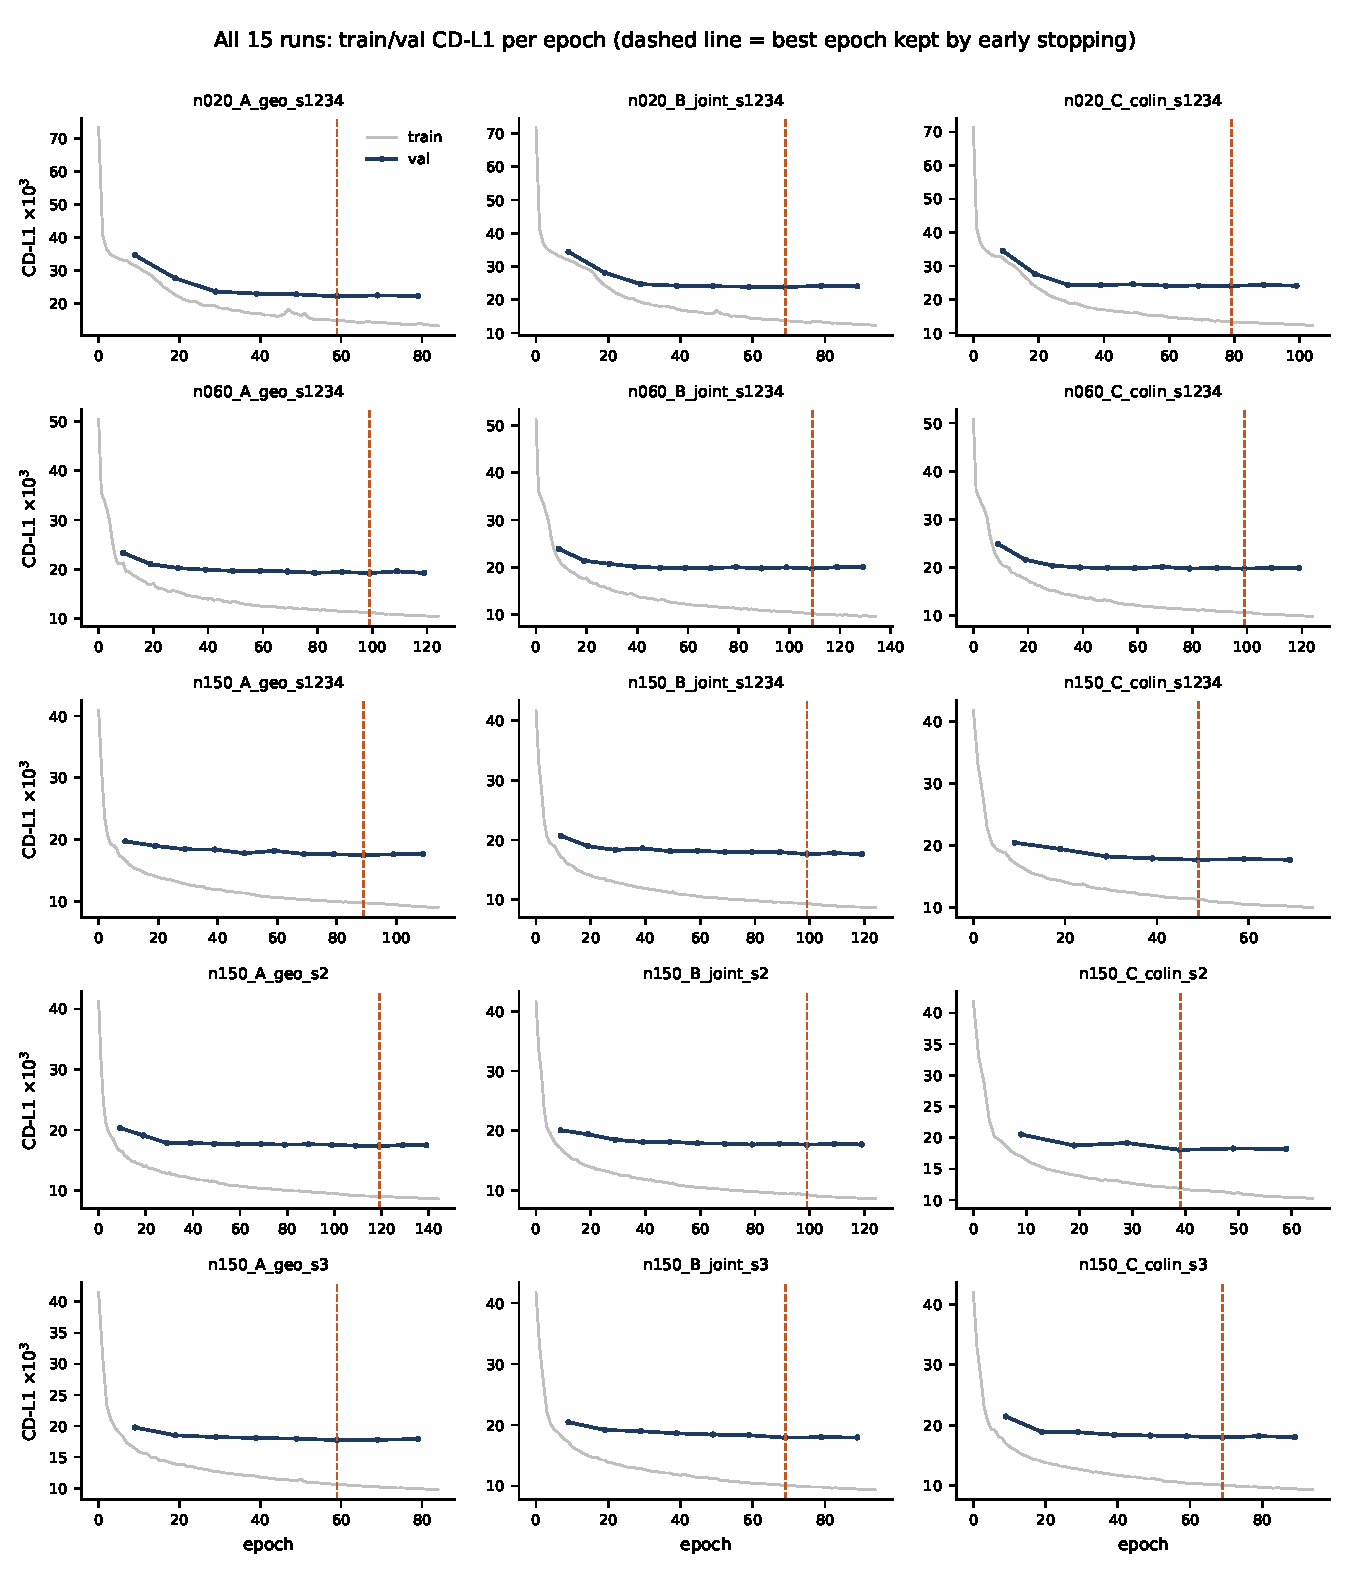
\includegraphics[width=0.94\textwidth]{figures/fig_training.pdf}
  \captionof{figure}{All \nRuns{} runs: train CD-L1 (gray) vs.\ validation CD-L1 (navy,
  every 10 epochs); the dashed line marks the best epoch whose checkpoint was kept.
  Validation plateaus early in every run while train keeps falling --- the data-limited
  signature motivating next week's proposals.}
\end{center}

\section{Provenance \& how to reproduce}\label{app:prov}

\begin{itemize}
  \item \textbf{Code:} \url{https://github.com/efeyenice/point-cloud-completion-research}
  --- the experiments ran from \texttt{main} at commit \texttt{ffa7bb3} (the \#8--\#16
  series). Model, splits, and drivers: \path{notebooks/pcnTraining.ipynb}. Data
  generation: \path{notebooks/partialGeneration.ipynb} + \path{tools/pc_resilient.py}.
  \item \textbf{Data + run artifacts:} HF dataset
  \href{https://huggingface.co/datasets/efeyenice/pc-completion-data}{\texttt{efeyenice/pc-completion-data}}
  at revision \texttt{\datasetRev}: \texttt{data/} (\nBundles{} \texttt{npz} bundles:
  8192-point colored GT + 8 partial views + metadata) and \texttt{runs/} (per-run
  \texttt{config.json}, \texttt{metrics.csv}, best/latest checkpoints,
  \texttt{curve.csv}, panels).
  \item \textbf{Live metrics:} W\&B project \texttt{pc-completion}, entity\\
  \texttt{efeyenice004-sabanc-university-nanotechnology-research-a}.
  \item \textbf{Model \& budget (from each run's \texttt{config.json}):} from-scratch PCN
  encoder--decoder, input 2048 points, coarse 1024, fine 8192; Adam, lr $10^{-4}$, step
  decay $\times 0.7$ every 50 epochs; batch 16; budget 300 epochs, early stop patience
  25 (val every 10); split seed 42; train seeds \{1234, 2, 3\}.
  \item \textbf{Reproduce:} open \texttt{pcnTraining.ipynb} on Colab (GPU), add
  \texttt{HF\_TOKEN} + \texttt{WANDB\_API\_KEY} to Secrets, run T0--T7 then T9 (the curve
  driver skips runs already on HF and resumes partial ones --- re-running is always
  safe), then T10 for figures/panels. This report:
  \texttt{make figures \&\& make} in \texttt{reports/2026-07-28-scale-curve/} --- every
  number in the prose is regenerated from the HF artifacts.
\end{itemize}

\section{Process log --- the week as it actually happened}\label{app:process}

\subsection*{Timeline}
\begin{itemize}
  \item \textbf{Jul 21--22.} Advisor meeting notes (compare architectures; explore color;
  more data; report numbers + visuals) distilled --- via a grilling session --- into one
  spine: the data-scale curve (ADR-0007). Harness built and locally validated: GPU FPS
  for partial generation ($\sim$8\,min $\rightarrow$ $\sim$5\,s/model, numpy fallback
  bit-identical), fixed test/val + nested train pools (unit-tested), color-copy
  baselines, early stopping, curve driver + report cells. PR \#8.
  \item \textbf{Jul 27 (morning).} Recurring pain --- Colab disconnects killing long runs
  and a growing Drive dependency --- triggered the research-ops decision (ADR-0008):
  git for code, HF for data + run artifacts, W\&B for metrics, Drive retired. Built and
  merged: resilient per-model data-gen module (\#10), HF-to-training loader (\#11),
  training wired to HF + W\&B (\#12), repo restructured for adopters + the co-research
  workflow written up (\#9, \#13, \#14).
  \item \textbf{Jul 27 (midday).} Data generation on Colab: \nBundles{} bundles streamed
  to HF. Incidents: a \texttt{NameError} (\texttt{NAME\_BY\_SYNSET} lived in a cell the
  run recipe skipped) fixed forward as \#15; one model failed mid-run --- the driver
  logged it, kept going, and the re-run picked it up (that is the resilience layer
  working as designed).
  \item \textbf{Jul 27 (afternoon).} Training gates passed on the new data; curve runs
  started. Mid-curve, the remaining single point of failure surfaced --- a VM recycle
  would have restarted the curve --- so the driver was made resumable from HF state
  (\#16) \emph{while the curve was running}, and the run continued across sessions.
  \item \textbf{Jul 27--28.} Top rung (9 runs) completed; \texttt{curve.csv} + panels
  landed on HF; this report built.
\end{itemize}

\subsection*{Incidents $\rightarrow$ lessons}
\begin{enumerate}
  \item \textbf{Runs died with the VM.} Lesson (now policy, ADR-0008): per-unit atomic
  commits to durable storage + idempotent resume, for \emph{every} long job. ``Done''
  means bytes on HF.
  \item \textbf{A skipped cell held a needed name.} Notebook cells form a hidden
  dependency graph; any cell a recipe skips must not define names others use. Fixed
  structurally in \#15.
  \item \textbf{Keep-alive $\neq$ resilience.} Headless/keep-alive running (colab-cli)
  reduces disconnects but cannot prevent VM eviction --- it complements, never replaces,
  resumability (\#16).
  \item \textbf{Secrets hygiene.} API keys were pasted into a chat transcript during
  setup; they were treated as compromised and rotated, and all notebooks read secrets
  from Colab Secrets/env only. Keys never enter git, notebooks, or reports.
\end{enumerate}

\section{Artifact map}\label{app:map}

\begin{center}\small
\begin{tabular}{ll}
\toprule
artifact & home \\
\midrule
code + notebooks (source of truth) & git --- \texttt{efeyenice/point-cloud-completion-research} \\
decisions + rationale & git --- \texttt{docs/adr/} (0001--0008), \texttt{CONTEXT.md}, \texttt{notes/} \\
method (how we co-research) & git --- \texttt{docs/WORKFLOW.md} \\
weekly reports & git --- \texttt{reports/} (this document) \\
generated datasets & HF dataset \texttt{efeyenice/pc-completion-data} (\texttt{data/}) \\
run artifacts (ckpts, metrics, curve) & same HF dataset (\texttt{runs/}) \\
live training metrics & W\&B project \texttt{pc-completion} \\
demo (planned) & HF Space \texttt{efeyenice/pc-completion-runs} \\
scratch / intermediates & Colab local disk (ephemeral by design) \\
\bottomrule
\end{tabular}
\end{center}

\end{document}
